\begin{abstract}
We look into the decidability of whether a hinged configuration locks.
\end{abstract}
\section{Introduction}
We look into the decidability of continuity on planar configuration space using regular, unitary hexagonal polygons.  These polygons can also represent unit disk configurations \cite{Breu19983} 
\begin{figure}[h]
\begin{center}
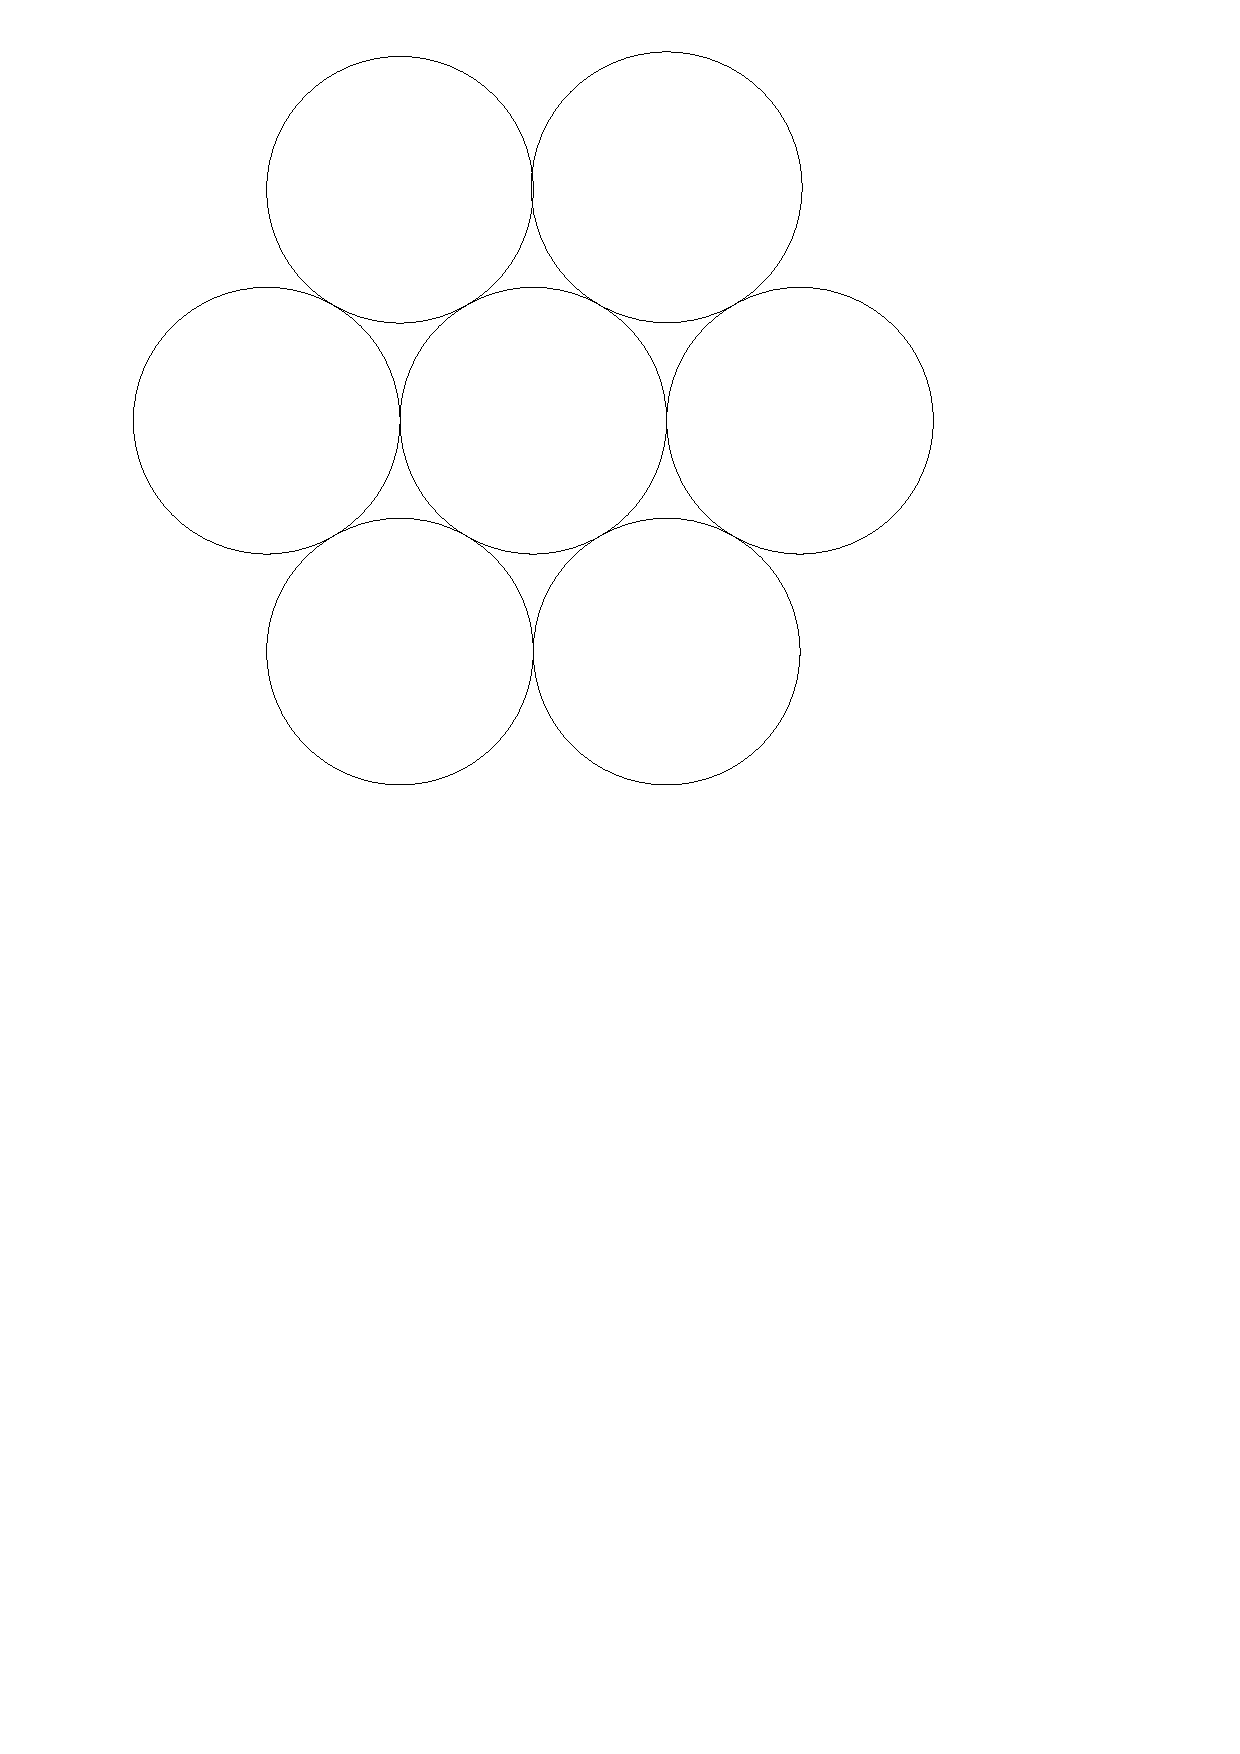
\includegraphics[scale=.5]{graphics/7ballLocked.pdf}
\caption{A locked 7 ball configuration}
\label{figure:7ballLocked}
\end{center} 
\end{figure}
% We need the following:
% \begin{itemize}
% \item[\rn{1}] discussion on the outer configuration of hexagons
% \item[\rn{2}] discussion on the inner configuration (lattice tesselation) of hexagons the convex hull of \rn{1}
% \item[\rn{3}] discussion on the hinged cells that reside in the boundary of \rn{2}
% \item[\rn{4}] discussion on the lockedness of \rn{3} where it has two modes (boolean variable)
% \item[\rn{5}] the area of interests:
% \begin{itemize}
% \item how big are the cells of \rn{3}?
% \item does cell size matter in \rn{3}?
% \item How to form a 3-sat conjunction from a set of cells at corners of the individual hexagons within the tesselation
% \item how to form a conjunction from a set of cells on the edges of the of the hexagons.
% \end{itemize} 
% \end{itemize}  
\paragraph{Motivation}
Protein folding, graphite, crystalline structures in metallurgy; disc packing;
hexagonal configurations;  Determine whether chemical structures are realizable.
\paragraph{Outline}
Section 2 covers the necessary mathematical concepts to understanding the
problem.  Section 3 explains the problem, Section 4 covers the results and
findings about the problem.  Section 5, the conclusion, offers final remarks on
the problem.
